\documentclass{article}

% Language setting
% Replace `english' with e.g. `spanish' to change the document language
\usepackage[english]{babel}

% Set page size and margins
% Replace `letterpaper' with `a4paper' for UK/EU standard size
\usepackage[letterpaper,top=2cm,bottom=2cm,left=3cm,right=3cm,marginparwidth=1.75cm]{geometry}

% Useful packages
\usepackage{amsmath}
\usepackage{graphicx}
\usepackage[colorlinks=true, allcolors=blue]{hyperref}

\title{{Algorithms SV worksheet 2}}
\author{Bálint Molnár}

\begin{document}
\maketitle


\section{Dynamic Programming}

\begin{enumerate}
    \item You are given $n$ boxes, so that the weight of the $i$-th box is $w[i]$ and the height of the box is $h[i]$. You would like to build a tower by putting some boxes on top of each other. However, you can only put box $A$ on top of box $B$ if $A$ has a smaller height and smaller weight. Design an algorithm to find the maximum height of such a tower.
    \item

    You are given an $N \times M$ grid. The field in row $i$ and column $j$ contains $A[i,j]\geq 0$ golden coins. Some fields are forbidden: If the field in row $i$ and column $j$ is forbidden, $B[i,j] = 1$; otherwise $B[i,j]=0$. Your goal is to go from the top left corner $(1,1)$ to the bottom right $(N, M)$, collecting as many coins as possible. In one step, you can move one step right or one step down. You are never allowed to move to forbidden fields.
    \begin{enumerate}
        \item Design an algorithm that finds the best route you can take (given $N, M, A, B$).
        \item How would you change your algorithm if you are allowed to move one step up as well? You won't get extra coins if you visit a field twice. You are also not allowed to leave the grid.
        \item What if you can move in all four directions?
    \end{enumerate}
    
    
    \item Recall that general trees can be defined in OCaml as
    \begin{verbatim}
        type 'a tree =
            | Node of 'a * 'a tree list
    \end{verbatim}

    Or equivalently as

    \begin{verbatim}
        class Tree<T> {
            T value;
            List<Tree<T>> children;
        }
    \end{verbatim}
    in Java.

    Design an algorithm that finds the longest path in the tree. See example below.\\ \emph{(please note that the longest path is not necessarily the longest downward path from the root, it may include both upwards and downwards steps)}
    \begin{figure}[h]
        \centering
        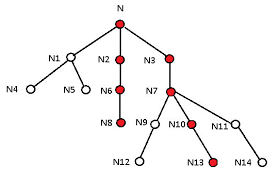
\includegraphics[width=0.32\linewidth]{longest-path.png}
        \caption{Q3: Longest path is labelled red}
        \label{fig:enter-label}
    \end{figure}
\end{enumerate}

\section{Greedy Algorithms}

\begin{enumerate}
    \item $N$ guests were invited. Each guest has indicated in advance the time intervals during which they will be present. The organisers want to capture all attendees in photographs during the event. Their goal is to take the minimum number of photos while ensuring that every guest appears in at least one photo.

    Design an algorithm that calculates the minimum number of photographs required and also determines the specific times when group photos should be taken.
    \item You are driving on a highway of length $L$ kilometres, with a car with  $T$ units of fuel tank capacity. Initially, the tank is full, and every kilometre uses $1$ unit of fuel. There are $N$ petrol stations, and the $i$-th station is $A[i]$ kilometres away from your starting point.
    \begin{enumerate} 
        \item Design an algorithm that, given $L, T, N, A$, finds the minimum number of times you need to refuel so you can get to the end of the highway, without running out of fuel. You can assume that all the inputs ($L,T, N,$ and elements of $A$) are integers and $A$ is sorted.
        \item Now assume that the price of fuel is $P[i]$ in the $i$-th station for each $i$. Design an algorithm that finds the minimum cost of fuel you need to get to the end of the highway (there is no limit on how many times you stop for refuelling).
    \end{enumerate}
\end{enumerate}

\end{document}